The Degree Planner UI layer consists of Web application, Course catalog, and Semester catalog. It is responsible for processing/displaying information related to degree planning tasks and interacting with the users. Important to notice, only authenticated users can access this layer.

\subsection{Layer Hardware}
The Degree Planner UI layer uses the screen of any devices having web browser(s).

\subsection{Layer Operating System}
The Degree Planner UI does not require any specific operating system since it is a web-based application running on any web browser.

\subsection{Layer Software Dependencies}
The Degree Planner UI is a web-based application built with ReactJS. It is implemented with React libraries, including react-beautiful-dnd and styled-component. React Router takes responsibility for navigating.

\subsection{Web Application}
Web application subsystem provides the user interface for the process of planning degree. The two fundamental goals of this layer is to display information and to interact with user. All courses corresponding to the users' major will be displayed in this UI. The users are capable of dragging course items and drop them into any semester columns.

%%%%%%%%%%%%%%%%%%%%%%%%%%%%%%%%%%%%%%%%%%%%%%%%%%%%%%%%%%
%  BE SURE TO UPDATE THE IMAGE CAPTION
\begin{figure}[h!]
	\centering
 	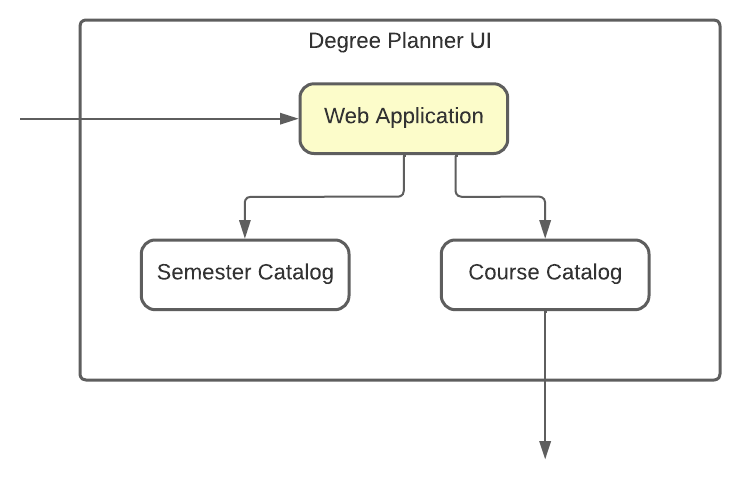
\includegraphics[width=0.60\textwidth]{images/WebApplication} % Image
 \caption{Web Application Subsystem} % Caption
\end{figure}

\subsubsection{Subsystem Hardware}
See section 3.1.

\subsubsection{Subsystem Operating System}
See section 3.2.

\subsubsection{Subsystem Software Dependencies}
See section 3.3.

\subsubsection{Subsystem Programming Languages}
This subsystem uses React with TypeScipt, and CSS.

\subsubsection{Subsystem Data Structures}
No particular data structure is required.

\subsubsection{Subsystem Data Processing}
Any data retrieved from Firestore database will be processed and formatted in Course and Semester subsystem. Web Application subsystem only receives the processed data from other subsystems and displays it to users.

\subsection{Course Catalog}
Course catalog subsystem fetches data from the database and sends it to the Web application subsystem. It is basically an interface between the Degree Planner UI layer and Firebase database layer.
%%%%%%%%%%%%%%%%%%%%%%%%%%%%%%%%%%%%%%%%%%%%%%%%%%%%%%%%%%
%  BE SURE TO UPDATE THE IMAGE CAPTION
\begin{figure}[h!]
	\centering
 	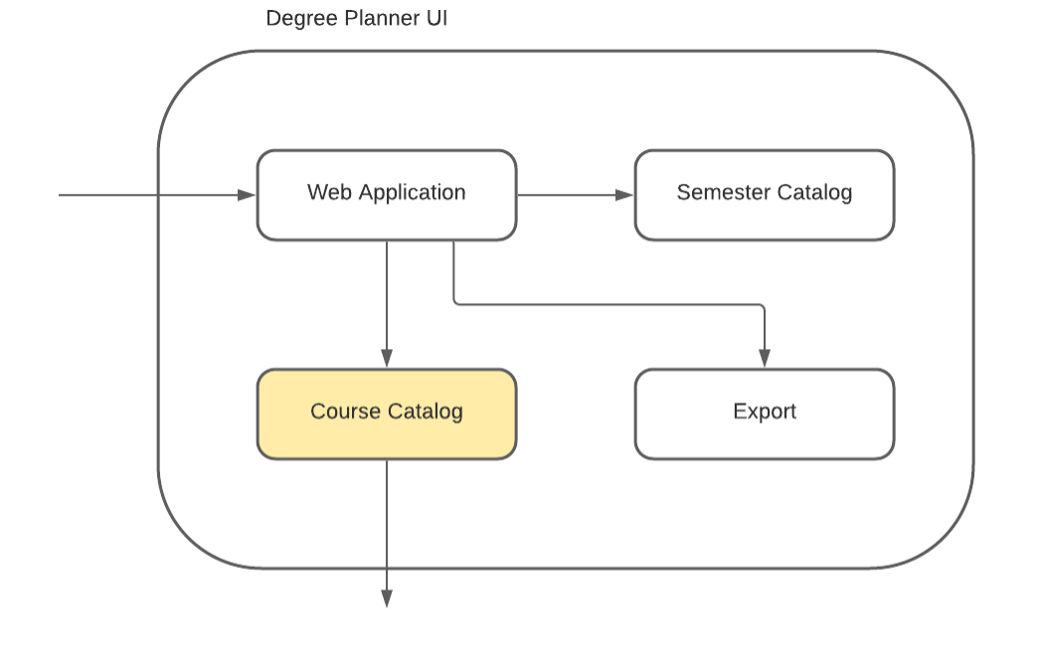
\includegraphics[width=0.60\textwidth]{images/CourseCatalog} % Image
 \caption{CourseCatalog Subsystem} % Caption
\end{figure}

\subsubsection{Subsystem Hardware}
See section 3.1.

\subsubsection{Subsystem Operating System}
See section 3.2.

\subsubsection{Subsystem Software Dependencies}
It will be implemented using the react-firebase library as well as Firestore database. For more information, see section 3.3.

\subsubsection{Subsystem Programming Languages}
This subsystem uses React with TypeScipt, and CSS.

\subsubsection{Subsystem Data Structures}
Each course retrieved from Firestore database into this subsystem has class Course. This user-defined object consists of nine properties, including document id, course id, course number, department, description, majors, availability, co-requisite, and pre-requisite courses. 

\subsubsection{Subsystem Data Processing}
This subsystem will receive data from Firestore database and process the data. It will then give that data to the web application subsystem. 

\subsection{SemesterCatalog}
Semester catalog subsystem reads data from the user information, and sends it to the Web application subsystem. It is basically an interface between UI layer and Dashboard layer. 

%%%%%%%%%%%%%%%%%%%%%%%%%%%%%%%%%%%%%%%%%%%%%%%%%%%%%%%%%%
%  BE SURE TO UPDATE THE IMAGE CAPTION
\begin{figure}[h!]
	\centering
 	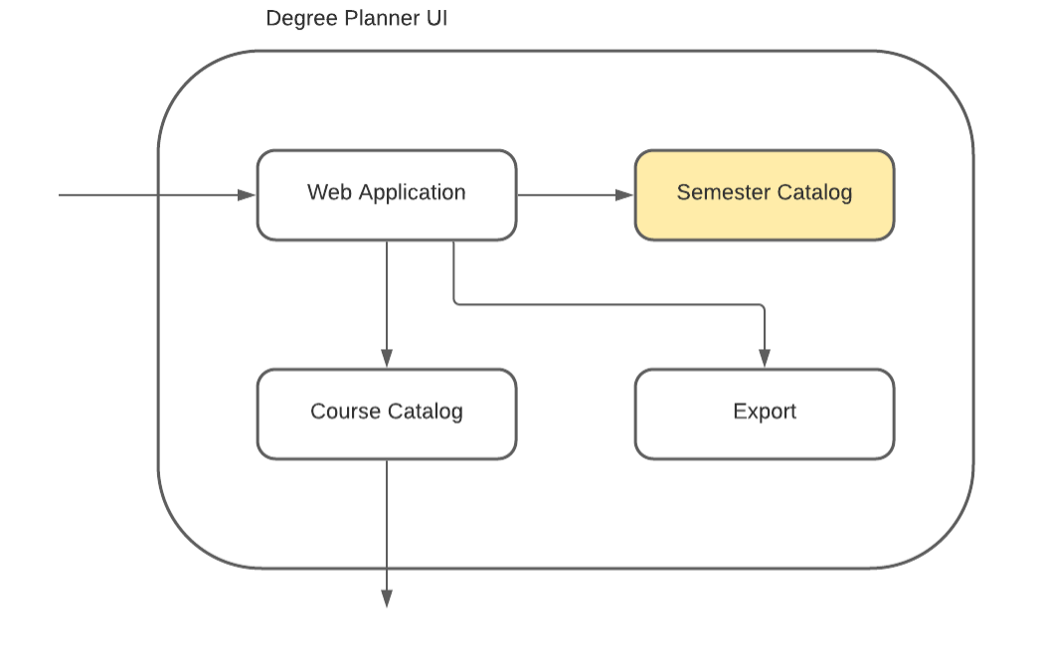
\includegraphics[width=0.60\textwidth]{images/SemesterCatalog} % Image
 \caption{SemesterCatalog Subsystem} % Caption
\end{figure}

\subsubsection{Subsystem Hardware}
See section 3.1.

\subsubsection{Subsystem Operating System}
See section 3.2.

\subsubsection{Subsystem Software Dependencies}
See section 3.3. 

\subsubsection{Subsystem Programming Languages}
This subsystem uses React with TypeScipt, and CSS.

\subsubsection{Subsystem Data Structures}
No particular data structure is required.

\subsubsection{Subsystem Data Processing}
This subsystem will read data and process the data into a Course object and send it to the web application system.

\vspace{100cm}










